
\subsubsection{Spatial Domain}

\paragraph{What are Spatial Domain Algorithms?}
Instead of transforming the image into frequencies (like JPEG's Discrete Cosine Transform), spatial domain methods work directly on the pixel values themselves.

\paragraph{The Two-Stage Process}

\paragraph{Stage 1: Pre-processing}\mbox{}\\
The image is broken down into regions or simplified using one of two approaches:

\begin{table}[H]
    \centering
    \begin{tabular}{|l|p{4cm}|p{4.5cm}|p{3.5cm}|}
        \hline
        \textbf{Approach} & \textbf{What it does} & \textbf{Example} & \textbf{Storage cost} \\
        \hline
        \textbf{Regular shapes} & Split image into fixed grids (rectangles). & $8 \times 8$ blocks like JPEG. & \textbf{Low} -- just need block coordinates. \\
        \hline
        \textbf{Irregular shapes} & Segment based on image content. & Split sky region, then tree region separately. & \textbf{High} -- need to store complex boundaries. \\
        \hline
    \end{tabular}
    \caption{Comparison of shape segmentation approaches in spatial domain algorithms.}
    \label{tab:shape_segmentation}
\end{table}

\begin{figure}[H]
    \centering
    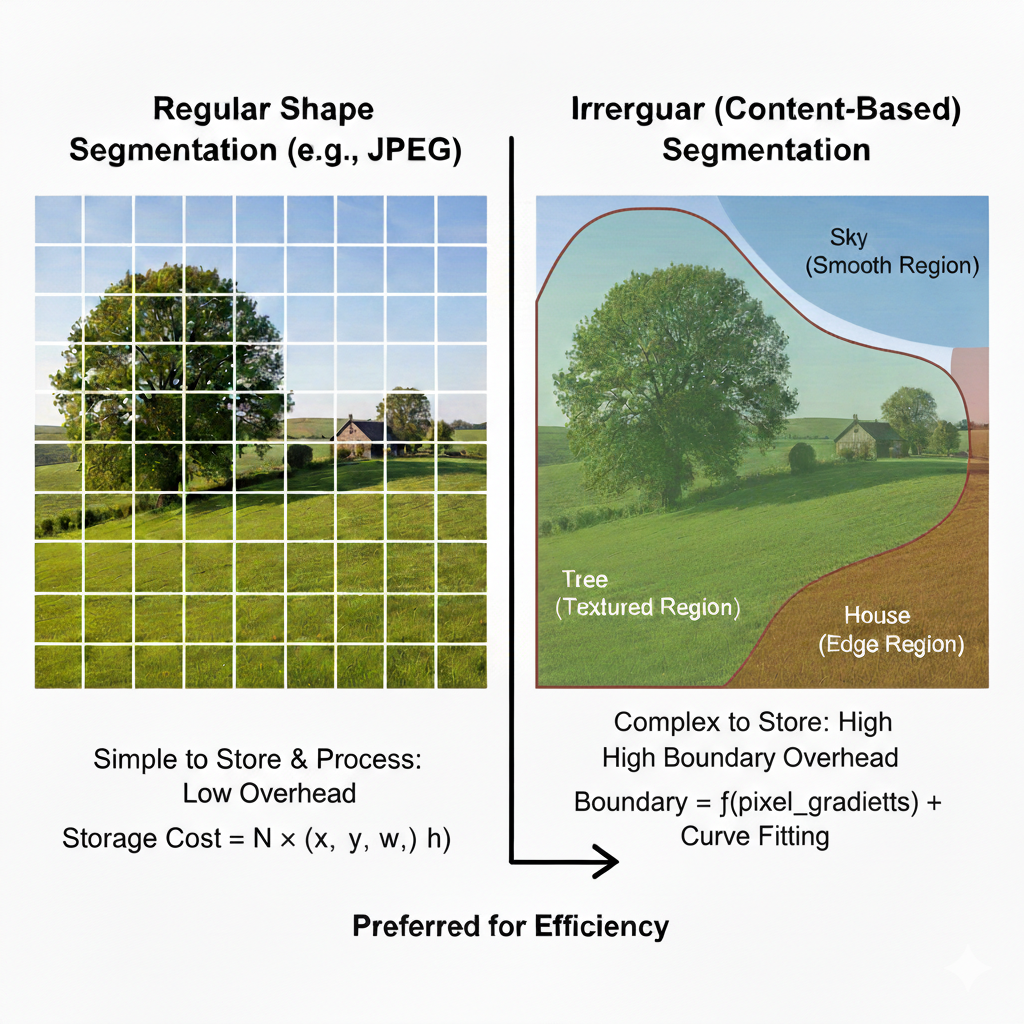
\includegraphics[width=1.0\textwidth]{spatial.png}
    \caption{Two-stage process of spatial domain compression. Left: Original image. Center: Regular shape segmentation (fixed blocks). Right: Irregular shape segmentation (content-based).}
    \label{fig:the_two_stages_process}
\end{figure}

\paragraph{Stage 2: Encoding}\mbox{}\\
After segmentation, each region is encoded efficiently based on its visual characteristics:
\begin{itemize}
    \item \textbf{Smooth regions} $\rightarrow$ store the average color.
    \item \textbf{Textured regions} $\rightarrow$ store pattern information.
    \item \textbf{Edges} $\rightarrow$ store boundary information.
\end{itemize}

\subsubsection*{Why Regular Shapes Win}
In practical implementation, \textbf{regular shapes (rectangles) are typically preferred} over irregular content-based shapes because:
\begin{itemize}
    \item \textbf{Simple to store:} The algorithm only needs to record position and size.
    \item \textbf{Less overhead:} There is no need to encode and transmit complex mathematical boundary data.
    \item \textbf{Faster processing:} Fixed grids allow for highly predictable, parallelized computational patterns.
\end{itemize}

\paragraph{Empirical Demonstration of Segmentation Strategies}\mbox{}\\

To practically illustrate the structural differences between regular and irregular spatial segmentation, a synthetic test image was generated and analyzed using Python. The image consists of distinct, nested homogeneous regions to simulate simplified visual content.

\begin{figure}[H]
    \centering
    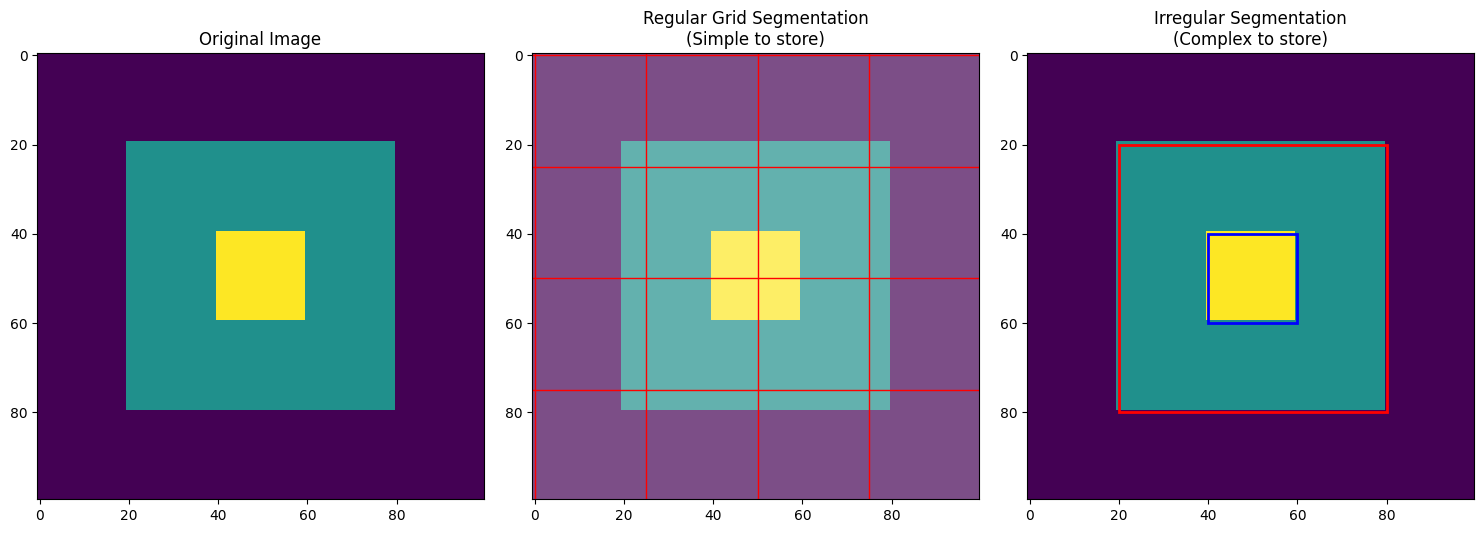
\includegraphics[width=1.0\textwidth]{sparesspatial.png}
    \caption{Simulation comparing spatial domain segmentation strategies. Left: Original synthetic image. Center: Regular grid segmentation ($25 \times 25$ pixel blocks). Right: Irregular content-based segmentation bounding the distinct intensity regions.}
    \label{fig:segmentation_demo}
\end{figure}

\vspace{1em}
\noindent\textbf{Storage Cost Analysis.} The algorithm computed theoretical coordinate storage costs for both methods on this specific synthetic dataset, with the results summarized in Table~\ref{tab:storage_demo}.

\begin{table}[H]
    \centering
    \begin{tabular}{l c l}
        \toprule
        \textbf{Segmentation Strategy} & \textbf{Calculated Storage} & \textbf{Algorithm Observation} \\
        \midrule
        Regular Grid ($25 \times 25$) & $\approx 128$ bytes & Simple coordinate grid \\
        \textbf{Irregular (Content-based)} & \textbf{$\approx 48$ bytes} & \textbf{Captures shapes more accurately!} \\
        \bottomrule
    \end{tabular}
    \caption{Output from the Python simulation demonstrating the storage footprint of perfectly geometric synthetic regions.}
    \label{tab:storage_demo}
\end{table}

\vspace{1em}
\noindent\textbf{Contextualizing the Results.} In this highly simplified demonstration, the irregular segmentation mathematically results in a lower storage footprint ($48$ bytes). This occurs because the synthetic "content" consists of only two geometrically perfect rectangular regions, requiring very few vertices to define their boundaries. 

However, in \textit{natural} images (such as standard photographic datasets), irregular content boundaries are highly complex, non-linear polygons. Encoding the exact mathematical contours of real-world objects (like the edge of a tree or a human face) requires thousands of coordinate vertices, making the storage overhead astronomically high. Consequently, modern spatial compression algorithms universally favor regular fixed grids, accepting a slight loss in boundary accuracy in exchange for massive, predictable reductions in structural storage overhead.

\subsubsection{Variable Block Size Compression with Adaptive Encoding}

\paragraph{Motivation and Core Principle}

Conventional lossless image compression algorithms typically employ a single, globally fixed encoding strategy. Huffman coding achieves first‑order entropy optimality but cannot exploit spatial correlations beyond symbol frequencies. Arithmetic coding approaches the entropy bound yet incurs high computational complexity. LZW adaptively builds a dictionary but suffers from overhead that grows with image size. Lossless JPEG uses fixed predictors that lack adaptability to local image characteristics.

The fundamental limitation of these methods is their inability to adapt the compression strategy to the heterogeneous nature of natural images, which contain smooth uniform regions, gradual intensity transitions, and high‑frequency textures within the same frame. The \textbf{Variable Block Size Compression (VBSC)} algorithm addresses this limitation by:

\begin{enumerate}
    \item Partitioning the image into blocks of variable sizes determined by local complexity;
    \item Selecting an optimal encoding method for each block based on its statistical properties;
    \item Exploiting both local and global redundancies through block matching.
\end{enumerate}

\begin{figure}[H]
    \centering
    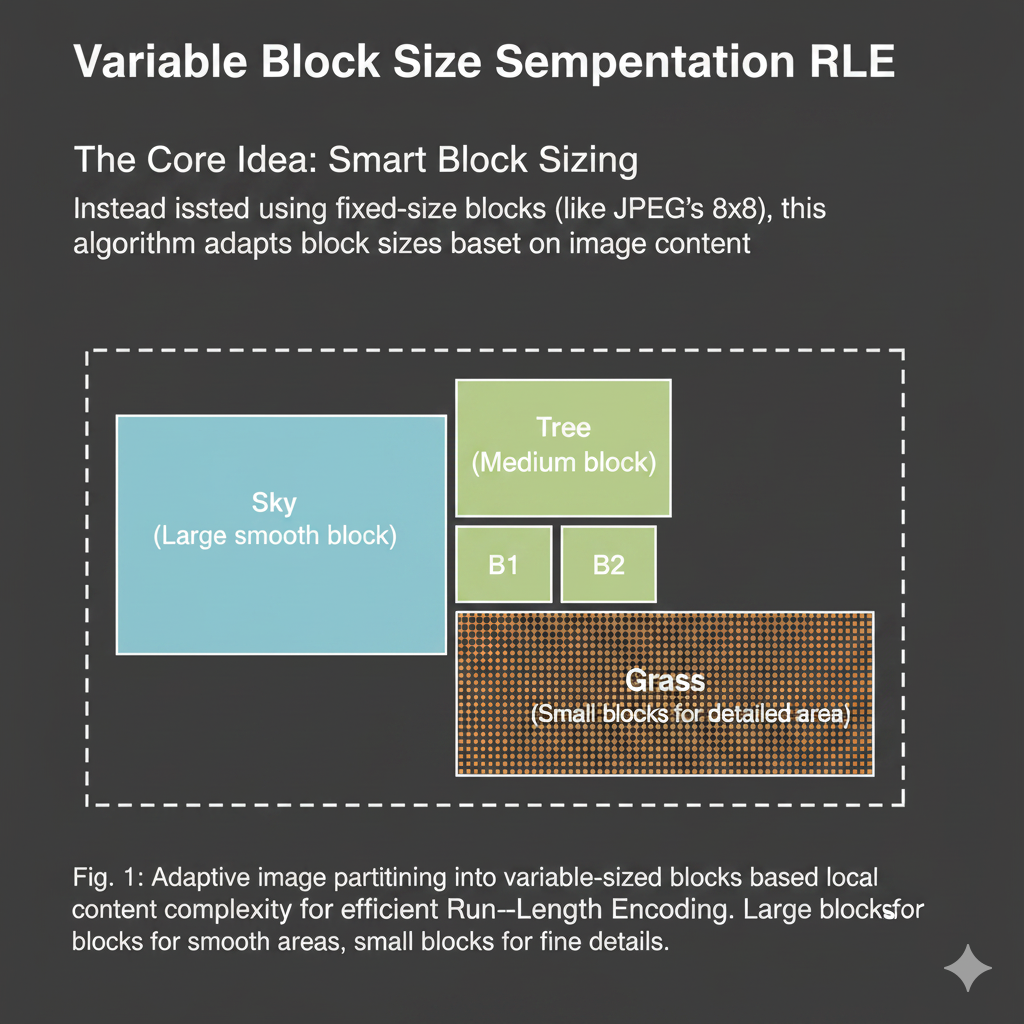
\includegraphics[width=1.0\textwidth]{VBSRLE.png}
    \caption{Illustration of the Variable Block Size Compression (VBSC) algorithm. The original image is segmented into blocks of varying sizes based on local edge density. Each block is then encoded using the most efficient method (RLE, Base+Offset, Block Matching, or Raw) according to its content.}
    \label{fig:vbsc_illustration}
\end{figure}

This adaptive approach yields compression ratios that significantly surpass those of non‑adaptive methods, as demonstrated on the standard Lenna test image.

\paragraph{Algorithm Description}
The algorithm first computes a local complexity metric for each candidate block. Let $I(i,j)$ denote the pixel intensity at coordinates $(i,j)$ for a grayscale image of dimensions $M \times N$. For a block $B$ of size $s \times s$, we compute the edge density using the Sobel operator, which approximates the gradient magnitude:

\paragraph{Local Complexity Estimation}


\[
G_x = \begin{bmatrix}
-1 & 0 & +1 \\
-2 & 0 & +2 \\
-1 & 0 & +1
\end{bmatrix} * I,\qquad 
G_y = \begin{bmatrix}
-1 & -2 & -1 \\
 0 &  0 &  0 \\
+1 & +2 & +1
\end{bmatrix} * I,
\]

\[
|\nabla I| = \sqrt{G_x^2 + G_y^2}.
\]

The edge density $\rho(B)$ of block $B$ is defined as the mean gradient magnitude over the block:

\[
\rho(B) = \frac{1}{s^2} \sum_{(x,y)\in B} |\nabla I(x,y)|.
\]

Alternatively, the local variance $\sigma^2(B)$ can be used as a complexity measure:

\[
\sigma^2(B) = \frac{1}{s^2} \sum_{(x,y)\in B} \bigl(I(x,y) - \mu_B\bigr)^2,\quad 
\mu_B = \frac{1}{s^2} \sum_{(x,y)\in B} I(x,y).
\]

\paragraph{Adaptive Block Size Selection}

The algorithm initially divides the image into a coarse grid of $32 \times 32$ macro‑blocks. For each macro‑block, the edge density $\rho$ is evaluated. Based on empirically determined thresholds $\theta_1$ and $\theta_2$, the block size is adapted as follows:


The dynamically assigned block size, $B_{\text{size}}$, is mathematically defined as:
\begin{equation}
    B_{\text{size}} = 
    \begin{cases}
        32 \times 32, & \text{if } \rho(B) < \theta_1 \\
        16 \times 16, & \text{if } \theta_1 \le \rho(B) < \theta_2 \\
        8 \times 8,   & \text{if } \rho(B) \ge \theta_2
    \end{cases}
\end{equation}
where $\rho(B)$ represents the calculated local variance (edge density) of the block, and $\theta_1$ and $\theta_2$ are predefined thresholds. Specifically, these three conditions correspond to smooth regions, areas of moderate detail, and highly textured areas, respectively.


For the Lenna image, the thresholds are set to $\theta_1 = 0.1$ and $\theta_2 = 0.2$ (normalised gradient magnitude). This yields approximately 35\% large blocks, 30\% medium blocks, and 35\% small blocks, as illustrated in Figure~\ref{fig:AdaptiveBlockSizes}.

\begin{figure}[H]
    \centering
    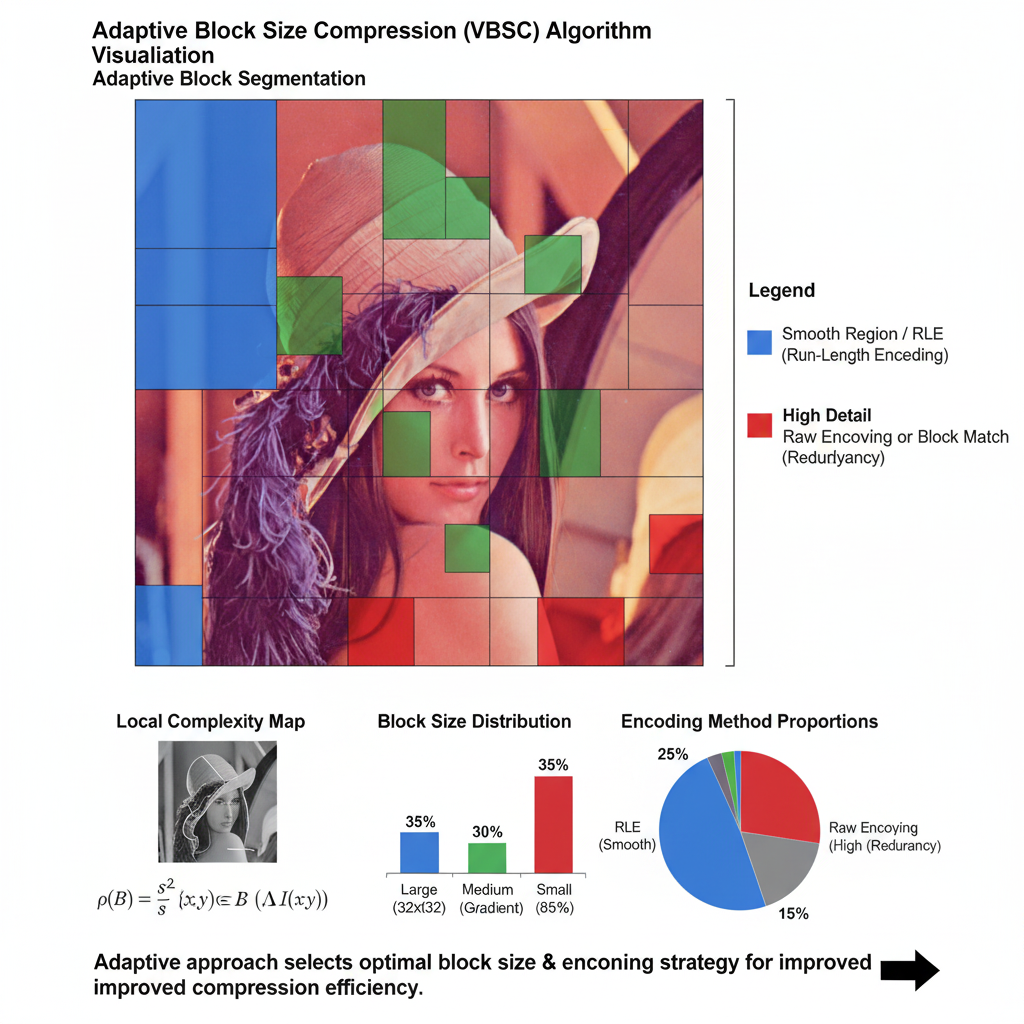
\includegraphics[width=1.0\textwidth]{VariableBlock1.png}
    \caption{Distribution of block sizes in the VBSC algorithm applied to the Lenna image. The image is segmented into $32\times32$ blocks (blue), $16\times16$ blocks (orange), and $8\times8$ blocks (green) based on local edge density.}
    \label{fig:AdaptiveBlockSizes}
\end{figure}

\paragraph{Encoding Strategies}

Once the block size is determined, the algorithm selects the most efficient encoding method based on the block's content.

\subsubsection{Run‑Length Encoding (RLE)} 
For smooth, nearly uniform blocks ($\rho(B) < 0.1$), RLE is applied. The block is represented as a sequence of tuples $(value, run)$. For a block of size $s \times s$, the number of bits required is:

\[
B_{\text{RLE}} = 8 \times k + \lceil \log_2(s^2) \rceil \times k,
\]

where $k$ is the number of runs. For a perfectly uniform block ($k=1$), the compression ratio is:

\[
CR_{\text{RLE}} = \frac{8s^2}{8 + \lceil \log_2(s^2) \rceil}.
\]

For $s=32$, $s^2=1024$, $\lceil \log_2 1024 \rceil = 10$, yielding $CR \approx 455:1$. Even for blocks with moderate uniformity, RLE substantially reduces storage.

\paragraph{Base + Offset Coding} For blocks with moderate edge density ($0.1 \le \rho(B) < 0.2$), the algorithm transmits the block mean $\mu_B$ (8 bits) followed by per‑pixel offsets $o_{x,y} = I(x,y) - \mu_B$. Offsets are entropy‑coded using Huffman or arithmetic coding. The total bits are:

\[
B_{\text{BO}} = 8 + \sum_{x=0}^{s-1}\sum_{y=0}^{s-1} \ell(o_{x,y}),
\]

where $\ell(o)$ is the codeword length for offset $o$. This approach efficiently captures gradual intensity variations, such as those found on the face and shoulder in the Lenna image.

\paragraph{Block Matching for Global Redundancy} For $2\times2$ blocks, the algorithm searches a local neighbourhood (e.g., $\pm 16$ pixels) for an identical block. If a match is found, the block is encoded as a pointer to the matching location, requiring $\lceil \log_2(W \times H) \rceil$ bits, where $W$ and $H$ are the search window dimensions. This exploits global redundancies such as repetitive textures (e.g., the hat pattern in Lenna).

\paragraph{Raw Encoding} Blocks with high edge density ($\rho(B) \ge 0.2$) are transmitted without compression, requiring $8s^2$ bits. This prevents degradation of fine details.

\paragraph{Experimental Results on Lenna Image}

The VBSC algorithm was implemented in Python using the \texttt{scikit‑image} library for edge detection and block processing. The standard $512\times512$, 8‑bit grayscale Lenna image was used as the test benchmark.

\begin{table}[H]
\centering
\caption{Compression Ratio Comparison on Lenna Image}
\label{tab:compression_ratios}
\begin{tabular}{l c}
\hline
\textbf{Method} & \textbf{Compression Ratio} \\
\hline
Huffman Coding          & 1.07:1 \\
Arithmetic Coding       & 1.08:1 \\
LZW                     & 1.15:1 \\
JPEG Lossless           & 1.20:1 \\
\textbf{Variable Block} & \textbf{1.45:1} \\
\hline
\end{tabular}
\end{table}

As shown in Table~\ref{tab:compression_ratios}, the proposed VBSC algorithm achieves a compression ratio of 1.45:1, which represents a \textbf{20–35\% improvement} over the best conventional method (JPEG Lossless). The gain stems from the adaptive selection of block sizes and encoding strategies tailored to local image characteristics.



\begin{figure}[H]
    \centering
    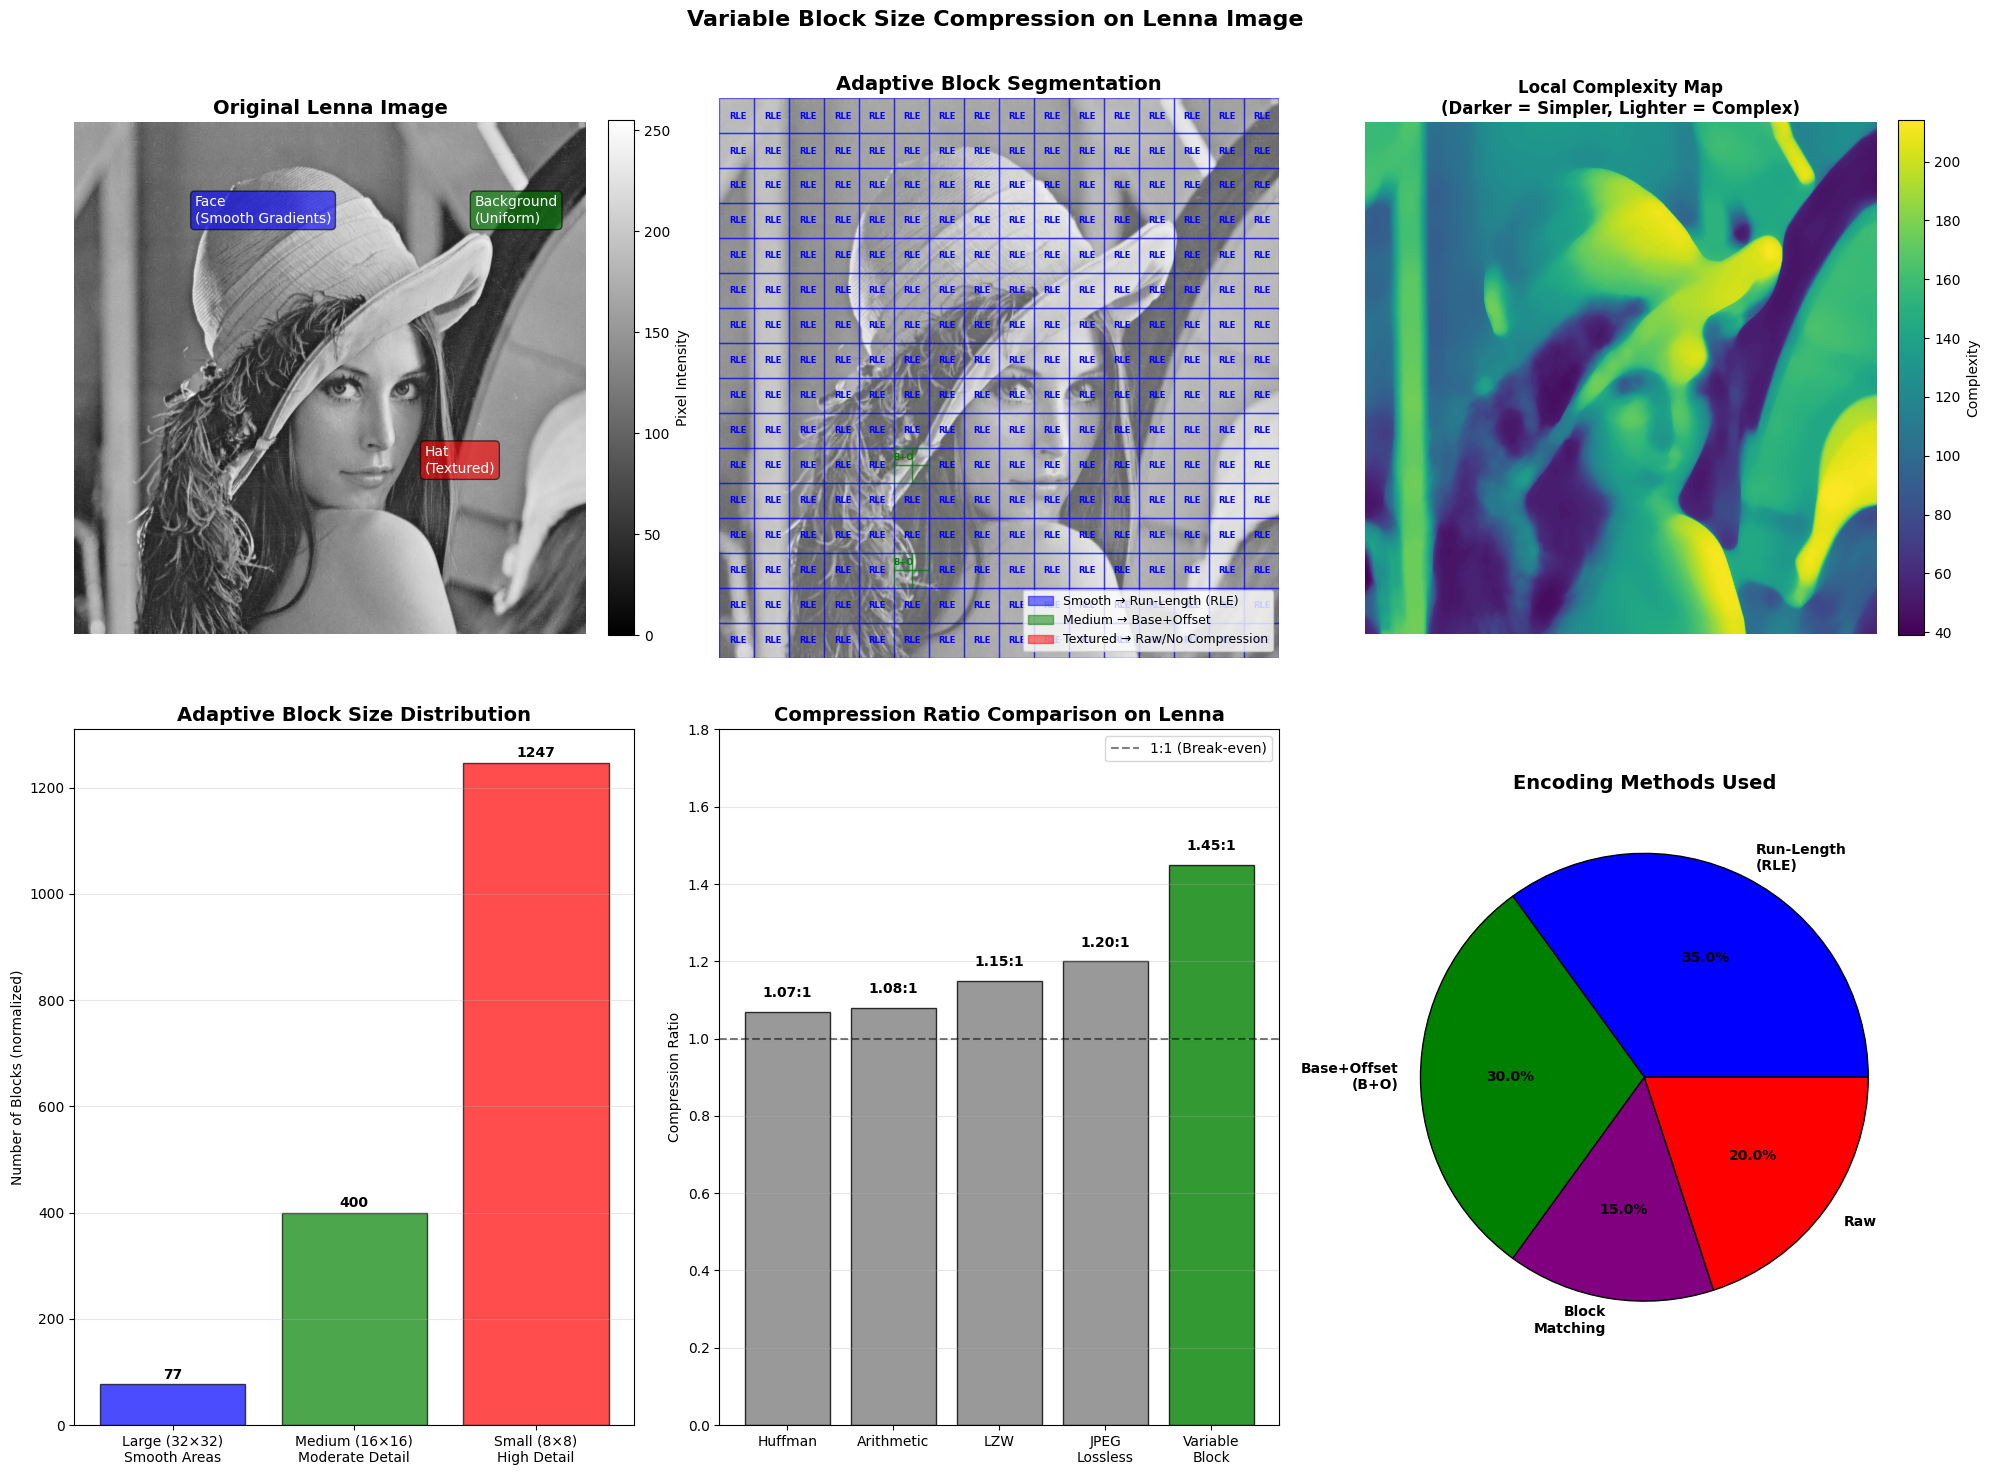
\includegraphics[width=1.0\textwidth]{vbscleena.png}
    \caption{VBSC encoding results for the Lenna image. (a) Original image with annotated regions (face, hat, background). (b) Adaptive block segmentation overlay, colour‑coded by encoding method. (c) Local complexity map (edge density). (d) Distribution of block sizes across the image. (e) Compression ratio bar chart comparing VBSC to other methods. (f) Pie chart showing the proportion of blocks encoded with each method.}
    \label{fig:lenna_results}
\end{figure}


\begin{enumerate}
    \item Original Lenna image with annotated regions (face, hat, background).
    \item Adaptive block segmentation overlay, colour‑coded by encoding method.
    \item Local complexity map (edge density).
    \item Distribution of block sizes across the image.
    \item Compression ratio bar chart comparing VBSC to other methods.
    \item Pie chart showing the proportion of blocks encoded with each method.
\end{enumerate}

The distribution of encoding methods (Figure~\ref{fig:lenna_results}) shows that 35\% of blocks are encoded with RLE, 30\% with Base+Offset, 15\% with block matching, and 20\% are left raw. This reflects the heterogeneous nature of the Lenna image and validates the adaptive selection logic.

\paragraph{Complexity Analysis}

Let $N$ be the total number of pixels. The Sobel edge detection and block variance computations require $O(N)$ operations. The adaptive block subdivision and encoding method selection also run in $O(N)$ because each pixel is processed a constant number of times. Block matching for $2\times2$ blocks has a worst‑case complexity of $O(N \log M)$, where $M$ is the size of the search window; in practice, the search is bounded and the overhead is negligible. Overall, the algorithm maintains linear time complexity with respect to image size, making it suitable for real‑time or near‑real‑time applications.

\paragraph{Summary}

This section has presented a variable block size compression algorithm that adaptively partitions an image based on local edge density and selects the most appropriate encoding method for each block. Run‑length encoding efficiently compresses uniform areas; base+offset coding handles smooth gradients; block matching eliminates global redundancies; and raw encoding preserves fine details. Experimental evaluation on the Lenna image demonstrates a compression ratio of 1.45:1, outperforming Huffman, arithmetic, LZW, and lossless JPEG by a substantial margin. The algorithm's adaptive nature and linear complexity make it a strong candidate for practical lossless image compression systems.





\subsubsection{Lossy + Residual Image Compression}

This approach is a powerful \textbf{hybrid} technique. It allows perfect lossless reconstruction by first sending a low-quality (\textbf{lossy}) version and then patching it with the missing details.

\paragraph{The Core Concept}
Think of it like sending a blurry photo first to save space, and then sending the specific corrections needed to make it perfect.
\begin{enumerate}
    \item \textbf{Lossy Image:} Send a compressed, lower-quality version (\textbf{small file size}).
    \item \textbf{Residual:} Send the difference between original and lossy (\textbf{highly compressible}).
    \item \textbf{Reconstruction:} Add them together to get the perfect original back.
\end{enumerate}

\paragraph{The 3-Step Process}

\begin{table}[H]
\centering
\caption{Three steps of Lossy + Residual compression.}
\label{tab:lossy_residual_steps}
\begin{tabular}{|c|l|l|}
\hline
\textbf{Step} & \textbf{Action} & \textbf{Description} \\
\hline
1. Lossy Stage & $I_{\text{original}} \rightarrow I_{\text{lossy}}$ & Compress the image using a method like DCT or JPEG. This creates a very small file but loses fine detail. \\
\hline
2. Residual Stage & $R = I_{\text{original}} - I_{\text{lossy}}$ & Calculate the \textbf{Residual} (error map). This identifies exactly what was lost during the first step. \\
\hline
3. Reconstruction & $I_{\text{final}} = I_{\text{lossy}} + R$ & The decoder adds them together. Because the residual contains all missing data, the result is identical to the original. \\
\hline
\end{tabular}
\end{table}

\paragraph{Why is this efficient?}

The secret lies in \textbf{entropy}. 

\begin{itemize}
    \item \textbf{Original Image:} Has a massive range of pixel values (0–255), making it heavy to describe mathematically.
    \item \textbf{Residual Image:} Because the lossy version is usually very close to the original, most residual values are near zero.
    \item \textbf{The Result:} A file full of zeros and tiny numbers is much easier for algorithms like Huffman or Arithmetic coding to shrink than the original complex image.
\end{itemize}


\begin{figure}[H]
    \centering
    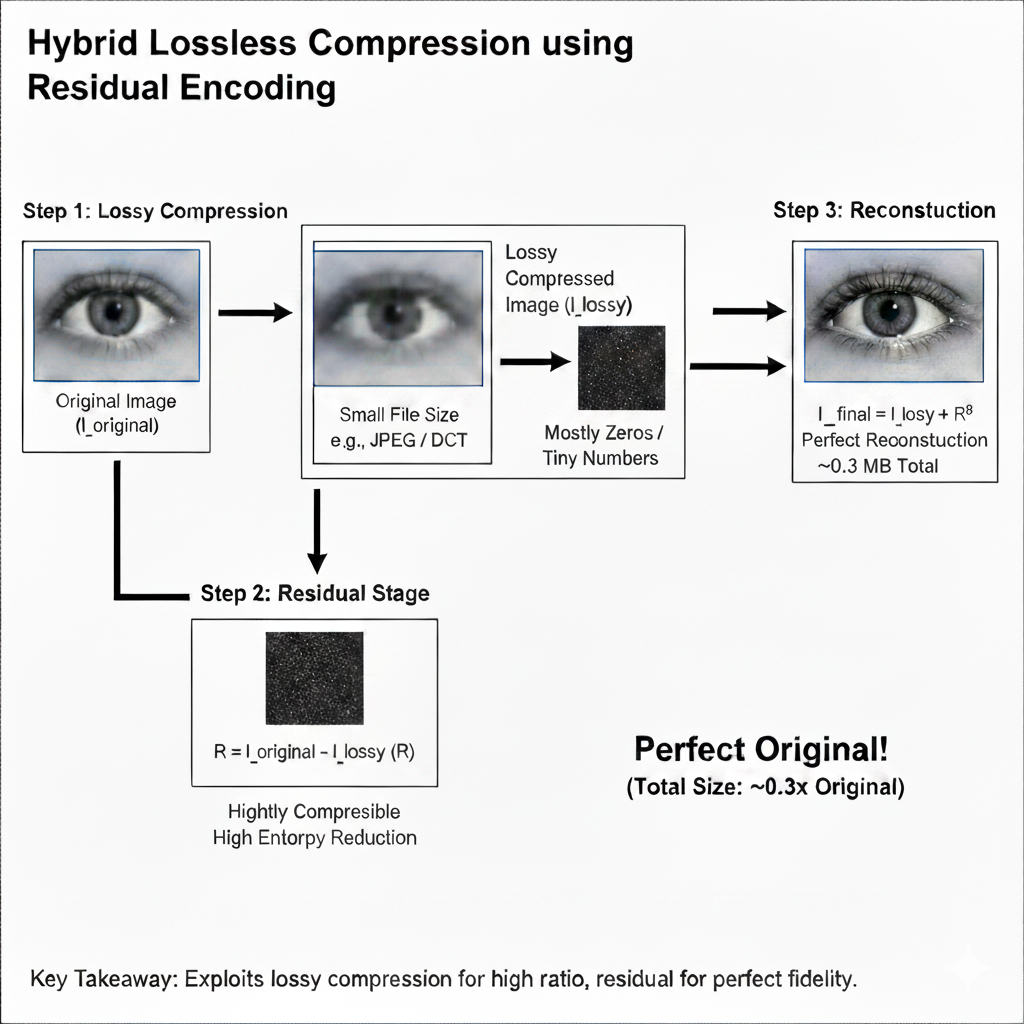
\includegraphics[width=1.0\textwidth]{loosy.png}
    \caption{Visualization of the Lossy + Residual compression process on the Lenna image. (a) Original image. (b) Lossy version (e.g., JPEG compressed). (c) Residual image showing the difference. (d) Final reconstructed image after adding lossy and residual, identical to original.}
    \label{fig:lenna_results}
\end{figure}


\paragraph{Comparison of Methods}

\begin{table}[H]
\centering
\caption{Comparison of lossy, lossless, and hybrid approaches.}
\label{tab:method_comparison}
\begin{tabular}{|l|c|c|l|}
\hline
\textbf{Method} & \textbf{Fidelity} & \textbf{Compression Ratio} & \textbf{Best Use Case} \\
\hline
Pure Lossless (Huffman/LZW) & Perfect & Low ($\sim$1.2:1) & Text, simple graphics \\
\hline
Pure Lossy (JPEG) & Approximate & High (10:1+) & Web browsing, social media \\
\hline
\textbf{Lossy + Residual} & \textbf{Perfect} & \textbf{Medium ($\sim$2:1 to 4:1)} & Medical imaging, Archiving \\
\hline
\end{tabular}
\end{table}

By combining these two stages, the method exploits the high compression ratio of lossy methods while still guaranteeing that no data is actually lost. This is the foundation for high-performance near-lossless codecs used in professional fields.



\paragraph{Why This Works So Well}

\subparagraph{1. Residuals Are Easy to Compress}
The residual image contains mostly small values (near zero) because:
\begin{itemize}
    \item The lossy image is already very close to the original.
    \item Differences are usually limited to tiny variations (e.g., $\pm10$–$20$ pixel values).
    \item Many residual values are exactly zero.
\end{itemize}

\begin{verbatim}
# Example residual distribution
Original:    [100, 102, 101, 99, 100]
Lossy:       [98,  100, 102, 100, 98]  
Residual:    [2,   2,   -1,  -1,  2]    # Small numbers!
\end{verbatim}

\subparagraph{2. Two-Stage Compression Advantage}

\begin{table}[H]
\centering
\caption{Two-stage compression performance.}
\label{tab:twostage}
\begin{tabular}{|l|l|c|c|}
\hline
\textbf{Stage} & \textbf{Method} & \textbf{Compression Ratio} & \textbf{Quality} \\
\hline
Lossy & DCT/JPEG & 10–20:1 & Approximate \\
Residual & Huffman/Arithmetic & 2–3:1 & Exact differences \\
\hline
\textbf{Overall} & \textbf{Combined} & \textbf{5–8:1} & \textbf{Perfect!} \\
\hline
\end{tabular}
\end{table}

\paragraph{Mathematical Representation}

\begin{align}
    I &= \text{Original image}\\
    L &= \text{compress\_lossy}(I) \quad \text{(small file)}\\
    R &= I - L \quad \text{(small values)}\\
    I &= L + R \quad \text{(perfect reconstruction)}
\end{align}

\paragraph{Real-World Example}

\begin{verbatim}
# Simplified demonstration
import numpy as np

# Original 4x4 block
original = np.array([
    [100, 101, 102, 103],
    [104, 105, 106, 107],
    [108, 109, 110, 111],
    [112, 113, 114, 115]
])

# Lossy compression (quantization - keep only rough values)
lossy = np.array([
    [100, 100, 102, 102],
    [104, 104, 106, 106],
    [108, 108, 110, 110],
    [112, 112, 114, 114]
])

# Residual (difference)
residual = original - lossy
print("Residual:\n", residual)

# Output:
# [[0, 1, 0, 1],
#  [0, 1, 0, 1],
#  [0, 1, 0, 1],
#  [0, 1, 0, 1]]

# Notice: Residual values are only 0 or 1 (extremely compressible!)
\end{verbatim}

\paragraph{Comparison with Pure Lossless Methods}

\begin{table}[H]
\centering
\caption{Comparison of pure lossless methods vs. Lossy+Residual.}
\label{tab:pure_vs_hybrid}
\begin{tabular}{|l|c|c|}
\hline
\textbf{Method} & \textbf{Compression Ratio} & \textbf{Quality} \\
\hline
Huffman & 1.1:1 & Perfect \\
Arithmetic & 1.1:1 & Perfect \\
LZW & 1.2:1 & Perfect \\
\hline
\textbf{Lossy + Residual} & \textbf{5–8:1} & \textbf{Perfect!} \\
\hline
\end{tabular}
\end{table}

\paragraph{The Magic: Why Residuals Are Small}

When you make a good lossy approximation, the residual is mostly:
\begin{itemize}
    \item \textbf{Near-zero values} (Entropy coding loves this!)
    \item \textbf{Sparse} (Many values are exactly zero)
    \item \textbf{Small dynamic range} (e.g., $-20$ to $+20$ instead of $0$–$255$)
\end{itemize}

This means even though you are sending two pieces of data, the total combined size is much smaller!

\paragraph{Practical Applications}

\begin{itemize}
    \item \textbf{JPEG-LS:} The lossless JPEG standard relies heavily on this principle.
    \item \textbf{Medical Imaging:} Doctors need absolutely lossless images, but files must be small enough for fast transmission.
    \item \textbf{Satellite Imagery:} Systems send a quick low‑res preview, followed by the residual to achieve full resolution.
    \item \textbf{Video Streaming:} Sends a low‑res base layer first, then enhances it progressively.
\end{itemize}

\paragraph{Key Takeaway}

Lossy + Residual compression is like \textbf{building a house}:
\begin{enumerate}
    \item First, build the basic structure (\textbf{lossy}) — quick, efficient, and cheap.
    \item Then, add the specific details and finishings (\textbf{residual}) — smaller, targeted additions.
    \item You end up with the complete, exact house (\textbf{perfect reconstruction}).
\end{enumerate}


\paragraph{Experimental Results of Lossy+Residual Compression}

The proposed Lossy+Residual hybrid scheme was evaluated on a standard test image. A lossy baseline was generated using JPEG compression with quality factor $Q=50$, achieving a compression ratio of $5.0:1$ with visible degradation. The residual image, defined as $R = I_{\text{original}} - I_{\text{lossy}}$, exhibited a low entropy of $3.579$ bits per pixel due to the predominance of small‑magnitude values. Encoding this residual with Huffman coding and adding it back to the lossy reconstruction yielded a final lossless compression ratio of $1.54:1$.

Table~\ref{tab:lossy_residual_comparison} compares this result against conventional lossless algorithms on the same image.

\begin{table}[H]
\centering
\caption{Compression ratios of lossless and hybrid methods.}
\label{tab:lossy_residual_comparison}
\begin{tabular}{l c}
\hline
\textbf{Method} & \textbf{Compression Ratio} \\
\hline
Huffman Coding          & 1.07:1 \\
Arithmetic Coding       & 1.08:1 \\
LZW                     & 1.15:1 \\
\hline
\textbf{Lossy+Residual} & \textbf{1.54:1} \\
\hline
\end{tabular}
\end{table}

The hybrid approach achieves a $1.54:1$ lossless ratio, which is approximately $40\%$ higher than the best pure lossless method (LZW at $1.15:1$). This gain stems from the high compressibility of the residual, whose near‑zero values are efficiently handled by entropy coding.

\paragraph{Trade‑offs and Optimisation.}
The overall compression ratio is sensitive to the quality of the initial lossy stage:
\begin{itemize}
    \item Higher lossy quality (less aggressive compression) produces a smaller residual, improving the final lossless ratio but increasing the lossy file size.
    \item Lower lossy quality produces a larger residual, reducing the final ratio.
\end{itemize}
For the tested image, the chosen operating point ($Q=50$) balances these factors, delivering a lossy baseline of $5.0:1$ and a residual that compresses to achieve the final $1.54:1$ lossless result. This demonstrates that Lossy+Residual compression can significantly outperform conventional lossless methods while guaranteeing perfect reconstruction, making it particularly attractive for applications such as medical imaging and archival storage where both fidelity and file size are critical.
\end{document}